%%=============================================================================
%% Verwerking resultaten
%%=============================================================================

\chapter{Verwerking Resultaten}
\label{ch:verwerking-resultaten}

\section{Analyse Resultaten Performantietesten}
\label{sec:analyse-performantietesten}

Bij een analyse van de resultaten valt onmiddellijk het verschil in de totale looptijd van de testen op: bij Cypress duurde het 565 seconden om de 5 testen te doorlopen, terwijl dit voor UFT 1185 seconden oftwel 109.7\% meer was.

Bekijken we de looptijden in detail, dan zien we dat er significante verschillen zijn tussen de testen onderling:

\begin{itemize}
    \item Factuur maken: 220 seconden vs. 225 seconden (2.3\% meer)
    \item Artikel toevoegen: 145 seconden vs. 195 seconden (34.5\% meer)
    \item Operator aanloggen: 60 seconden vs. 255 seconden (325\% meer)
    \item Handscanner gebruiken: 50 seconden vs. 285 seconden (470\% meer)
    \item Betaling registreren: 90 seconden vs. 210 seconden (133.3\% meer)
\end{itemize}

Het is niet onmiddellijk duidelijk hoe deze verschillen verklaard kunnen worden. Sowieso lijken de testen die gebruik maken van randapparaten (``handscanner gebruiken'' en ``betaling registreren'') meer tijd in beslag te nemen in de UFT implementatie. Dit kan te maken hebben met de gebruikte simulator, maar dit zou onderzocht moeten worden.

Volgende tabel toont de verschillende maten van elk van de metrieken voor \textbf{Cypress}:

\begin{longtable}{llllll}
          & Private Bytes & Private MB & \% Processortijd & Thread Count & Handle Count \\
\endhead
%
Min.      & 828600320     & 790        & 0.0              & 55           & 4347         \\
Q1        & 2651780096    & 2529       & 22.6             & 525          & 14583        \\
Avg.      & 2661191393    & 2538       & 93.6             & 519          & 14265        \\
Med.      & 2698608640    & 2574       & 126.3            & 531          & 14656        \\
Q3        & 2767050752    & 2639       & 153.5            & 535          & 14718        \\
Max.      & 2878648320    & 2745       & 234.6            & 550          & 15243        \\
Std. Dev. & 228128244     & 218        & 69.3             & 54           & 1327        
\end{longtable}

De resultaten voor \textbf{UFT} zijn als volgt:

\begin{longtable}{llllll}
          & Private Bytes & Private MB & \% Processortijd & Thread Count & Handle Count \\
\endhead
%
Min.      & 339161088     & 323        & 0.0              & 89           & 4740         \\
Q1        & 1941017600    & 1851       & 3.2              & 271          & 9578         \\
Avg.      & 1929173402    & 1840       & 21.8             & 264          & 8972         \\
Med.      & 1963698176    & 1873       & 15.6             & 286          & 9679         \\
Q3        & 2054377472    & 1959       & 25.6             & 302          & 9763         \\
Max.      & 2132299776    & 2034       & 151.8            & 334          & 10244        \\
Std. Dev. & 242146684     & 231        & 28.2             & 63           & 1652        
\end{longtable}

De meest interessante gegevens zijn wellicht het geheugengebruik en gebruik van processortijd. Voor beide kandidaat frameworks zijn de grafieken hiervoor onder te vinden:

\begin{figure}[h!]
    \centering
    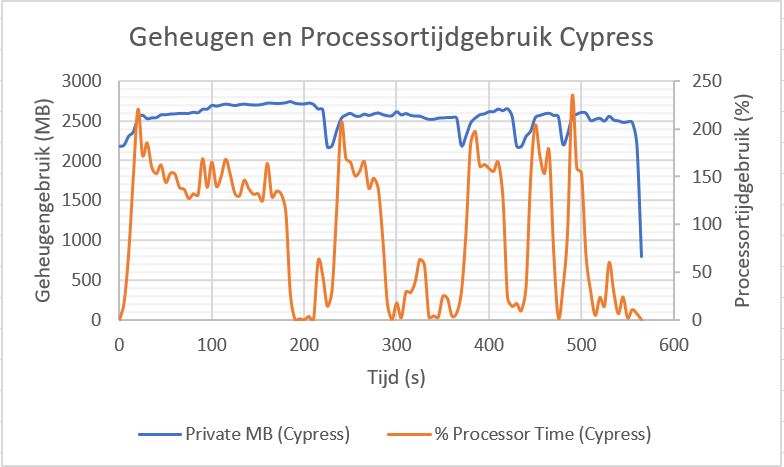
\includegraphics[scale=0.6]{img/resultaten/processor-geheugengebruik-cypress.PNG}
    \caption{Gebruik van geheugen en processortijd tijdens uitvoer van de testen voor Cypress}
    \label{fig:resultaten-cypress}
\end{figure}

\begin{figure}[h!]
    \centering
    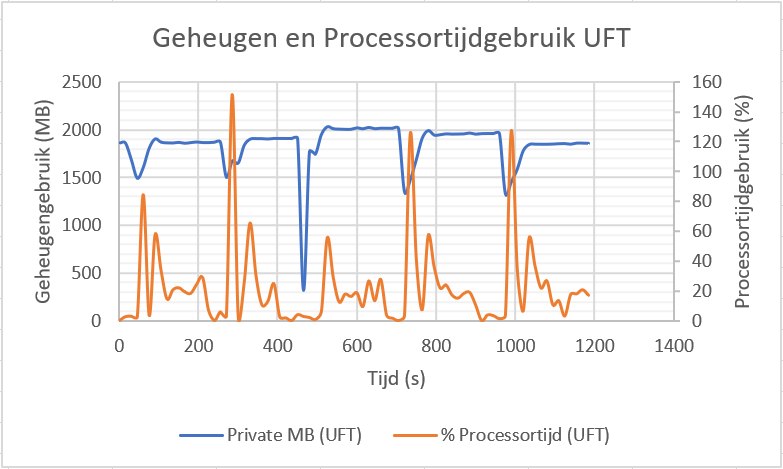
\includegraphics[scale=0.6]{img/resultaten/processor-geheugengebruik-uft.PNG}
    \caption{Gebruik van geheugen en processortijd tijdens uitvoer van de testen voor UFT}
    \label{fig:resultaten-uft}
\end{figure}

Opvallend is dat Cypress beduidend meer geheugen gebruikt dan UFT. De standaardafwijkingen bevinden zich in dezelfde grootteorde en ook visueel kunnen we zien dat het geheugengebruik vrij stabiel is (behalve aan het einde van een test). De conclusie is dus dat Cypress meer geheugen gebruikt dan UFT. Echter doet UFT er meer dan dubbel zo lang over om de testen uit te voeren. Een hoger geheugenverbruik is zeker een aanvaardbaar nadeel indien dit een kortere doorlooptijd als gevolg heeft — zeker indien het end-to-end testen op een apart toestel plaatsvindt.

Qua processortijd gebruik blijkt Cypress opnieuw de computer zwaarder te belasten met een gemiddelde van 93,6\% tegenover 21,8\% voor UFT. De spreiding is ook significant groter bij Cypress (standaardafwijking van 69,3\%) dan bij UFT (28,2\%). Opnieuw kunnen we hier hetzelfde stellen: het gebruiken van een groter percentage van de beschikbare processortijd is niet \emph{in se} problematisch, indien dit een snellere uitvoering van de testen als resultaat heeft.

Thread en handle count liggen bij Cypress ook hoger dan bij UFT, hoewel de standaardafwijkingen voor beide relatief dicht bij elkaar liggen en UFT zelfs een grotere mate van spreiding vertoont. Logischerwijze is dit echter gecorreleerd met het geheugengebruik.

\section{Resultaten Requirements}
\label{sec:resultaten-requirements}

De drie kandidaat frameworks voldoen allen in grote mate aan de vooropgestelde requirements. Hieronder worden de voornaamste punten herhaald:

\begin{itemize}
    \item \textbf{Protractor} wordt ontwikkeld door Google, hetzelfde bedrijf dat ook Angular ontwikkeld. Dit wil zeggen dat de kans dat de ontwikkeling van Protractor onverwachts stopgezet wordt, vrij klein is. De software is open source (wat betekent dat er geen dure licentiekosten zijn) en zou vrij vlot aan te leren zijn. Voor deze kandidaat werden helaas geen praktijktesten uitgevoerd en dus kan de performantie niet vergeleken worden met de andere frameworks. Bovendien vereist het framework Selenium en WebDriver JS om te kunnen runnen.
    \item \textbf{Cypress} is een jong framework dat specifiek voor Angular ontwikkeld werd, hoewel het ook voor andere webapplicaties gebruikt kan worden. Het vereist geen andere software om te werken en kan vrij snel aangeleerd worden. Het framework is snel in het uitvoeren van testen en kan geïntegreerd worden in de IDE die door Colruyt Group gebruikt wordt. Bovendien is het open source en dus 'gratis'. Daarentegen staat het framework nog in zijn kinderschoenen; het framework kan in de toekomst drastische veranderingen ondergaan en/of de ontwikkeling kan stopgezet worden. Dit is een reëel risico.
    \item \textbf{UFT} is een zeer krachtig en veelzijdig framework dat reeds binnen Colruyt Group gebruikt wordt (Colruyt India). Het biedt een brede waaier aan functionaliteiten, en kan voor elk type client-server applicatie gebruikt worden. Bovendien is de kans klein dat de ontwikkeling ervan binnenkort stopgezet wordt. Daarentegen is UFT veel trager in het uitvoeren van testen, is de leercurve heel steil, en zijn de licenties duur.
\end{itemize}